\documentclass{report}
\usepackage{graphicx}
\usepackage{amsmath}
\usepackage{indentfirst}
 
\begin{document}
 
 \begin{titlepage}
	\centering
    
\includegraphics[width=4cm, height=3cm]{head-white-gray-big.png}

	{\scshape\LARGE Washington State University \par}
	\vspace{1cm}
	{\scshape\Large Computer Science 322\par}
	\vspace{1.5cm}
	{\huge\bfseries Requirements Specification\par}
	\vspace{2cm}
	{\Large\itshape David Harkins\par}
	\vfill
	Instructor\par
	\textsc{Neil Corrigan}

	\vfill
	{\large \today\par}
\end{titlepage}
\pagebreak
 
\tableofcontents{}
\pagebreak

\listoffigures

\section*{Revision History}

\begin{description}
\item[Revision 2, \today]: Updated based on peer review feedback. 
\item[Revision 1, March 11, 2016]: The initial version of the requirements specification.
\end{description} 
\pagebreak



\iffalse Section 1: Introduction ---------------------------- \fi
\chapter{Introduction}
 	The purpose this document is to define the Turing machine simulation program. Also to provide a structured and uniform set of requirements for use during the development of this application. Finally this document contains the functionality agreed upon by the client and the developer. This will be used to determine when the application meets the standards and is complete. The audience for this document is the developer, David Harkins, future developers, and the client, Neil Corrigan. 
    
    This document will cover general background information about and provide an overview to the problem that the software is attempting to solve. The formal definition of a Turing machine, which was created by Alan Turing, will be given and explained for a quick overview of syntax. Next the document will cover the environment that the application runs in. This includes in which context for which the application will run. Next it will cover the file formats for the Turing machine definition file and the input string file. For both file types, examples will be provided, and strict rules are also defined in the description. It will also cover the steps that are required to start the Turing machine application and the steps to terminate the application. Finally the usage and commands are defined and examples are provided for how the user will interact with the application. Each of the commands it to have a description of what they are for and how they work. Each command is labeled with the character required to invoke the command. Also examples are provided of a user using the command and the result that will be achieved. 
  
    
    
\iffalse Section 2: Background ---------------------------- \fi
\chapter{Background}
 	A Turing machine is an abstract mathematical model of a computer. It manipulates symbols on an infinite tape according to specific rules defined in each Turing machine. For any algorithm, a Turing machine can be constructed to represent the logical steps, and simulated to produce the same result. A Turing machine is specified by it's formal definition $M = (Q, \Sigma, \Gamma,\delta,q_0 , B, F)$, Where:\newline
    
  
   
\begin{itemize}
\item $Q$ is a finite set of states
\item $\Sigma \subseteq $ ( $\Gamma$ - {B}) is a finite input alphabet
\item $\delta$ is a transition function from Q $\times \space \Gamma \rightarrow$ Q $\times \space \Gamma \times \left\{L, R\right\}$
\item $q_0 \in$ Q is the initial state
\item B $\in$ $\Gamma$  is the blank symbol
\item F $\subseteq$ Q is the set of final states
\end{itemize}
    
A string x $\in$ $\Sigma$* is accepted by M if $q_0$x $\vdash$ $\alpha_1$$p$$\alpha_2$ for some $p$ $\in$ $F$ and $\alpha_1$$\alpha_2$ $\in$ $\Gamma$*. Otherwise, the string is rejected.
\pagebreak
    \begin{figure}[!ht]
  		\centering
   		 \
      	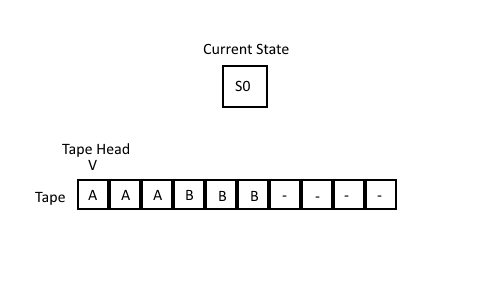
\includegraphics[scale=1]{TM_Example_Tape.png}
  \caption{Example of a running turing machine}
\end{figure}

\begin{itemize}
\item Current State: The that the Turing machine is in.
\item Tape Head: The current cell the Turing Machine is pointing at. The Turing machine can only change the character in the cell that the tape head is pointing at.
\item Tape: Contains a group of cells that have a single character contained within. 
\end{itemize}


\pagebreak
    
\iffalse Section 3: Overview ---------------------------- \fi
\chapter{Overview}
 	The purpose of the Turing machine software is to simulate a valid Turing machine on user provided input strings. The Turing machine is loaded from a definition file with a specific formatting and containing all of the parts of the formal definition. The input strings are loaded from an input string file and also can be entered during execution by the user. To run the Turing machine simulator the user will execute the executable with the name of the Turing machine definition file without the extension provided as the first and only command line argument. A response message will be displayed to the user on the result of loading the Turing machine definition file. Upon failure to load the definition file named the same as the command line argument an error message will be displayed and the application will quit. Upon successfully loading a definition file named, the same as the command line argument, the application will display a successful message and prompt for a command. The application will prompt the user to enter a command until the user enters the exit command. If any changes where made to the input string file that was loaded into memory, the application will attempt to save the file. A message will be displayed with the result of the attempt, and the application will exit.
   
   	\pagebreak
    \begin{figure}[!ht]
  		\centering
   		 \
      	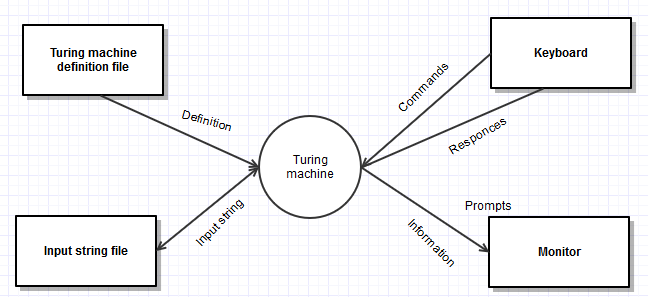
\includegraphics[scale=0.85]{context.png}
  \caption{The context within which the application will operate.}
\end{figure}

    
\iffalse Section 4: Environment ---------------------------- \fi
\chapter{Environment}
 
\section{Input and Output Devices}
The user provides input through the use of a standard keyboard. The output is to the standard display which is the user's monitor (See figure 3.1). 
\section{Turing Machine Definition File}

The Turing machine definition file contains eight main parts. The separation between each part is marked with a keyword. The keywords are required to be in the order listed below. Each element in the definition file must be separated by at least one white space. There is no limit on the number of white space separating the elements which makes the definition file not dependent on the formatting. All of the text between the keywords is classified as the part of the section the last keyword indicated. The keywords can be in upper case, lower case or any mixture of both. A definition file will be considered erroneous if any of the following occur in the definition file: If the file is missing any of the keywords or they are in a incorrect ordering; If any of the sections is missing information before transiting to the next; If any of the requirements for the sections below are not met. The following is the list of parts and keywords that appear in the Turing machine definition file in the order they must be in.

\begin{enumerate}
\item Description (no keyword) - There is no keyword, all of text before the second section is the description. The description is commonly the definition of what the Turing machine accepts but is not limited to it.

\item States (STATES:) - This section contains the list of state names where each state name is unique.

\item Input Alphabet (INPUT\_ALPHABET:) - This section contains the list of input characters where each input character is unique. This cannot contain the bracket characters or the arrow characters.

\item Tape Alphabet (TAPE\_ALPHABET:) - This section contains the list of tape characters where each tape character is unique. The tape alphabet must contain the blank character and also the input alphabet. The this cannot contain the bracket characters or the arrow characters.

\item Transition functions (TRANSITION\_FUNCTION:) - This section contains the list of the transition for the Turing machine. The parts that make a transition must contain elements from the list of states and tape alphabet.

\item Initial state (INITIAL\_STATE:) - The starting state of the Turing machine. This state must be in the list of states.

\item Blank character (BLANK\_CHARACTER:) - The character that represents the blank character. This cannot be contained within the input alphabet.

\item Final States (FINAL\_STATES:) - The final states for the Turing machine. Each state must be contained within the list of states.

\end{enumerate}



\begin{verbatim}
Example of a Turing machine definition file:

This Turing machine accepts the language of one or more a's 
followed by the same number of b's.

STATES: s0 s1 s3 s4

INPUT_ALPHABET: a b

TAPE_ALPHABET: a b X Y -

TRANSITION_FUNCTION:
  s0 a   s1 X R
  s0 Y   s3 Y R
  s1 a   s1 a R
  s1 b   s2 Y L
  s1 Y   s1 Y R
  s2 a   s2 a L
  s2 X   s0 X R
  s2 Y   s2 Y L
  s3 Y   s3 Y R
  s3 -   s4 - R
  
INITIAL_STATE: s0

BLANK_CHARACTER: -

FINAL_STATES: s4
\end{verbatim}


\section{Input String File}

The format for the input string file is an input string on each line and the backslash character for a blank character. The extension for the input string file must be .str. The input string file is evaluated line by line and if a single line is rejected as invalid the remaining lines are not necessarily rejected. If a line contains any character that is not in the input string the line is rejected.

\begin{verbatim}
Example of the input string file: 

a
ab
\
aaabb
aaaaaaaaaabbbbbbbbbb
aabb
aaaaaabbbbbbb
ba
aba
bb
\end{verbatim}    
    
\iffalse Section 5: Operation ---------------------------- \fi
\chapter{Operation}

	At the beginning of operation the Turing machine simulation will check for one and only one command line argument. If there is no command line argument or it is more than one the application prints an error message and terminates. If it is a single argument, the application attempts to load a Turing machine definition file. The name of the file is specified by the user's command line argument with a .TM appended to it. If a file does not exist by that name, or the application is unable to read it, an error message is displayed and the program terminates. If the definition file is loaded into memory successfully, it will validate the Turing machine definition file. If the validation fails, an error message is displayed, and the application terminates. If the validation is successful, a message will be displayed to the user, and another file will be attempted to be loaded. This is the input string file which was specified by the user's command line argument with a .STR appended to it. If there is no file by that name, or it is unable to be read, the application will continue without any error message. If the application is able to load the file, it will validate the content. If there are any invalid lines they will be removed and a message displayed to the user. If the application loads the input string file without any validation errors, no message will be displayed to the user. Next, the application repeatedly prompts the user for a command. For a list of commands and usage see the sections below.

\par
At the time the user enters the command 'exit', which is specified by the character 'x', the application will do the ending task. If the input string file was modified by removing invalid strings on loading, the user entered a new string, or the user deleted a string, the application will attempt to save the file. On the 'exit' command, the new version of the file modified by the user will overwrite the original file. The application will display a message of the results from attempting to write the file to disk and terminate.
 
\section{Invocation}

\subsection{Command Line} 
To successfully run the Turing machine simulation program, the user must provide a single command line argument when starting the application. Failure to provide a single argument will result in a error message and the termination of the program. If a single command line is provided to the application, it will attempt to load a Turing machine definition file. The file's name is the command line argument with the extension .TM appended to it. If the Turing machine definition file is not found, or cannot be read an error message is displayed and the application terminates. Upon successfully loading a Turing machine file by said name, it will be validated. If the validation fails an error message is displayed and the application terminates. If the validation is successful a message will be displayed to the user and another file will be attempted to be loaded. This is the input string file which was specified by the user's command line argument with a .STR appended to it. If there is no file by that name, or it is unable to be read the file, application will continue without any error message. If the application is able to load the file, it will validate the content. If there are any invalid lines, they will be removed, and a message displayed to the user. If the application loads the input string file without any validation, errors no message will be displayed to the user.

\begin{verbatim}
Example of running the application with a command line argument:

$ TM Definition
\end{verbatim}

\subsection{Configuration Settings} 
The application has default values for the two changeable settings. The default values are set upon the start of the application and they are not preserved across uses of the application. The first setting is the number of transitions to do per run command (see below for details on run command). The default setting for this is one transition. The next setting is the number of tape characters to display before truncating. The default value is 32 but these settings can be changed by the user using the commands below. 

\subsection{Opening Turing Machine} 
If a single command line is provided to the application it will, attempt to load a Turing machine definition file. The file's name is the command line argument with the extension .TM appended to it. If the Turing machine definition file is not found, or cannot be read, an error message is displayed, and the application terminates. Upon successfully loading a Turing machine file by said name, it will validate it. If the validation fails, an error message is displayed and the application terminates. If the validation is successful, a message is displayed to the user, and the application continues.

\section{Commands}

The following are the possible commands that the user can enter to trigger events in the application. The input from the user must be one of these commands, no other input is allowed unless actively using one of the commands.

\subsection{Help User (specified by h)} 

The help command is used by the user to get a list of valid commands and their descriptions. 

\begin{verbatim}
Example of using the help command:

Command: h

(D)elete   - Delete input string from list.
E(x)it     - Exit application.
(H)elp     - Help user.
(I)nsert   - Insert input string into list.
(L)ist     - List input strings.
(Q)uit     - Quit operation of Turing machine on input string. 
(R)un      - Run Turing machine on input string.
S(e)t      - Set maximum number of transitions to perform. 
Sho(w)     - Show status of application.
(T)runcate - Truncate instantaneous description.
(V)iew     - View Turing machine.

Command: 
\end{verbatim}

\subsection{Show Status (specified by w)} 

\begin{verbatim}
Example of using the show command:

Command: w

Course name: CPT_S 322
Semester: Spring
Year: 2016

Instructor: Neil Corrigan
Author: David Harkins

Version number: 1
Max transitions: 10
Max cells to left and right: 10
Name of TM: A
TM Status: Completed
The input string aaabb has been accepted in 7 transitions.
    
Command: 
\end{verbatim}

\subsection{View Turing Machine (specified by v)} 

The view command is used to view the currently loaded Turing machine definition file.

\begin{verbatim}
Example of using the view command:

Command: v

This Turing machine accepts the language 
of one or more a's followed by the same number of b's.

Q = {s0, s1, s2, s4}
	
Sigma = {a, b}

Gamma = {a, b, X, Y, -}

Delta(s0, a) = (s1, X, R)
Delta(s0, Y) = (s3, Y, R)
Delta(s1, a) = (s1, a, R)
Delta(s1, b) = (s2, Y, R)
Delta(s1, Y) = (s1, Y, R)
Delta(s2, a) = (s2, a, R)
Delta(s2, X) = (s0, X, R)
Delta(s2, Y) = (s2, Y, R)
Delta(s3, Y) = (s3, Y, R)
Delta(s3, -) = (s4, -, R)

Q0 = s0

B = -

F = {s4}


Command: 
\end{verbatim}

\subsection{List Input Strings (specified by l)} 

The command list is used to display the input strings that the user can run the Turing machine on. Each input string is displayed with a sequential index number and on it's own line. If the input string is a blank character, the line will display the number and a backslash. If there are no strings to list, a message to this effect will be displayed to the user.

\begin{verbatim}
Example of using the list command:

Command: l

1. a
2. ab
3. \
4. aaabb
5. aaaaaaaaaaabbbbbbbbbb
6. aabb
7. aaaaaabbbbbbb
8. ba
9. aba
10. bb

Command: 
\end{verbatim}

\subsection{Insert Input String (specified by i)} 

The insert command allows the user to enter a new string that is not already on the list that consists of the input alphabet. If the string is invalid, an error message is displayed, and the application prompts for a new command. If the input string is valid, the application adds the new string to the list, sets the flag to overwrite the input string file, displays a message to the user, and prompts for a new command. If the user does not enter a string, the command is terminated without any messages, and the application prompts for a new command. If the user enters a backslash, the application adds a empty string to the list.

\begin{verbatim}
Example of using insert command:

Command: i

Input string: abbb
String inserted into list!
    
Command: 
\end{verbatim}

\subsection{Delete Input String (specified by d)} 
The delete command allows the user to delete a single input string from the list. The user enters the index number of the string to specify which string to delete. If the index corresponds to a string it is deleted and all of the rest of the strings are renumbered, a success message is displayed to the user, and the application prompts for a new command. If the provided index does not correspond to a valid string index, the application displays an error and prompts for a new command. If the user does not enter a string index, the command is terminated without any message displayed and the application prompts for a new command.
\begin{verbatim}
Example of using the delete command:

Command: d

Input string number: 1
String deleted!

Command: 
\end{verbatim}

\subsection{Set Transitions (specified by e)} 

The set command allows the user to change the setting for the maximum number of transitions to be performed at a time during the operation of a Turing machine on an input string. When the command is invoked, the current setting is displayed to the user, and the user is prompted to enter a new value that is at least one. If the value is valid, a message is displayed, the setting is changed and the user is prompted for a new command. If the value is less than one, a fraction or a decimal number an error is displayed, and the command is terminated prompting the user for a command. The default value for this setting is one and is set at run time. If the user does not enter any value, the command is terminated, and the application prompts for a new command.

\begin{verbatim}
Example of using the set transition command:

Command: e
Maximum number of transitions [1]: 20
Number of transitions changed to 20.
    
Command: 
\end{verbatim}

\begin{verbatim}
Example of an error while using the set transition command:

Command: e
Maximum number of cells [1]: -1
Error: A non-numerical input entered.    
Command: 
\end{verbatim}

\subsection{Truncate Instantaneous Descriptions (specified by t)} 

The truncate command sets the maximum amount of tape cells on the left and on the right to display before truncating. The default value for this setting is 32 which is set at run time. If the user enters a number greater than one, a message is displayed, the setting is changed, and the user is prompted for another command. If the value is less than one, a fraction or a decimal number an error is displayed, and the command is terminated prompting the user for a command. 

\begin{verbatim}
Example of using the truncate command:

Command: t

Maximum number of cells [32]: 10
Setting changed!
    
Command: 
\end{verbatim}

\subsection{Run Turing Machine (specified by r)} 

The run command will start the simulation of a Turing machine on an input string or continue the simulation of a Turing machine on a input string. If there is not a Turing machine running, the user is prompted for an input string index. If the user enters nothing, the command is terminated and the user is prompted for a another command. If the input value is less than one, a fraction or a decimal number an error is displayed and the command is terminated prompting the user for a command. If the input index is valid, a Turing machine simulation is started with that input string. The initial state is displayed with the input string and the current state in square brackets at the corresponding position on the tape. The state is displayed and with all of the characters to the left of where the tape head is pointing on the left side of the state and everything to the right of where the tape head is pointing, including the tape cell currently pointed at, on the right side of the state. If the right or left side is longer than the maximum length before truncation, the left or right side will be truncated, and an arrow will be placed to indicate that is was truncated. This is referred to as the instantaneous description of the Turing machine. If the tape is empty, only the state will be displayed. The Turing machine will simulate until the amount of transitions reaches the maximum transitions or the input string is accepted or rejected. If it is accepted or rejected, a message will be displayed with the input string, if it accepted or rejected, and the number of transitions. At this point the instantaneous description of the Turing machine will be printed out, and the user will be prompted to enter a command. 

\par If the run command is invoked and a Turing machine is still being simulated, the machine will be simulated until the maximum amount of transitions is reached, or the input string is accepted or rejected. If it is accepted or rejected a message will be displayed with the input string, if it accepted or rejected and the number of transitions.




\begin{verbatim}
Example of using the run command:

Command: r

Input string number: 1
0. [s0]aaabb
7. XXXXY-[s4]
Input string aaabb was accepted in 7 transitions.

Command: 
\end{verbatim}

\subsection{Quit Turing Machine (specified by q)} 

The quit command terminates operation on a Turing machine simulation. A message is displayed to the user of how many transitions were preformed and the input string. If the application is not currently running on a Turing machine simulation an error message, is displayed to the user.

\begin{verbatim}
Example of using the quit command:

Command: q

Input string aaabb was not accepted or rejected in 112 transitions.

Command: 
\end{verbatim}

\subsection{Exit Application (specified by x)} 
 The exit command terminates the Turing machine simulation application program. If the input string file was changed the application, will attempt to save it over the existing one. The result will be displayed to the user and regardless of success or failure the application will close.
 
\begin{verbatim}
Example of using the exit command:

Command: x

Input string file successfully saved to disc.

$ 
\end{verbatim}

\section{Termination}

\subsection{Closing Turing Machine} 
At the time the user enters the 'exit' command, which is specified by the character 'x', the application will do the ending task. If the input string file was modified by removing invalid strings on loading, the user entered a new string, or the user deleted a string, the application will attempt to save the file. The new version on save will overwrite any existing file. The application will display the results from attempting to write the file to disk to the display and terminate.
 

\iffalse Section References: ---------------------------- \fi
\chapter{References}

\begin{itemize}
\item Neil Corrigan - General notes, lecture and help.
\end{itemize}

 

 
\end{document}

